\documentclass[11pt,a4paper]{article}
\usepackage[T2A,T1]{fontenc}
\usepackage[utf8]{inputenc}
\usepackage[english,russian]{babel}
\usepackage{geometry}
\usepackage{graphicx}
\usepackage{booktabs}
\usepackage{microtype}
\usepackage[hidelinks]{hyperref}
\geometry{margin=22mm}
\graphicspath{{results/}}
\setlength{\parindent}{1.25em}
\setlength{\parskip}{0.25em}
\newcommand{\code}[1]{{\fontencoding{T1}\selectfont\ttfamily #1}}

\title{EDM-анализ обучения Muon/nanoGPT на FineWeb10B}
\author{Технический отчёт по файлу \code{message (2).txt}}
\date{30 июля 2026 г.}

\begin{document}
\maketitle

\begin{abstract}
Из самодокументируемого текстового лога восстановлен один полный запуск
Muon/nanoGPT: 2330 последовательных значений training loss и 11 значений
validation loss. Для плотного ряда проведена фазовая реконструкция и
скользящая оценка intrinsic dimension методом Levina--Bickel. В отличие от
экспериментов с grokking, выраженного позднего коллапса размерности не найдено.
После удаления локального тренда оценка остаётся около 10--10.5 на основной
части обучения. Эксперимент следует интерпретировать как контрольный пример,
демонстрирующий важность detrending и проверки стационарности.
\end{abstract}

\section{Исходный эксперимент и извлечение данных}

Файл содержит полный код обучения, описание окружения и собственно лог. Парсер
использует только строгие маркеры \code{RUNMETA}, \code{RUNEND}, записи
\code{train\_loss} и \code{val\_loss}; исходный файл не изменяется.

Восстановлен запуск \code{Muon\_lr0.06\_5db64adc}: 12-слойный GPT
(model dimension 768, 6 attention heads) обучался на FineWeb10B с Muon
(learning rate 0.06, momentum 0.95, weight decay 0) на 8 NVIDIA H100. Глобальный
batch равен 262144 токенам, основной цикл содержит 2290 итераций и 40
дополнительных. Linear learning-rate cooldown начинается примерно с шага 1260.
Запуск завершился без дивергенции за 143.8 секунды; итоговый validation loss
равен 3.2785.

Training loss в исходном логе является усреднённой между GPU суммой потерь по
локальному батчу. Для получения средней token-level cross-entropy он делился на
$262144/8=32768$. Полученный ряд непрерывен на шагах 0--2329.

\begin{figure}[ht]
  \centering
  
\includegraphics[width=\textwidth]{01_training_overview.pdf}
  \caption{Training и validation loss вместе с learning-rate schedule.}
\end{figure}

\section{Методика EDM}

EDM применялся только к training loss: 11 validation-точек недостаточно для
фазовой реконструкции. Использовались окна длиной 400 шагов со сдвигом 40.
В каждом окне задержка выбиралась по первому локальному минимуму delayed mutual
information, после чего строилось embedding размерности 12. Intrinsic dimension
оценивалась методом Levina--Bickel по 10 соседям. Для исключения тривиальной
временной близости применялось Theiler window шириной 12 шагов.

Анализ повторялся после удаления локального линейного тренда. Это необходимо,
поскольку быстрое монотонное снижение loss образует почти одномерную кривую в
delay space и может искусственно занизить оценку размерности.

Для прямой сопоставимости воспроизведён estimator из существующего проектного
кода: embedding dimension 15, $k=5$, $\tau=1$, без Theiler window. Его
абсолютные значения выше, однако качественная динамика совпадает.

\begin{figure}[ht]
  \centering
  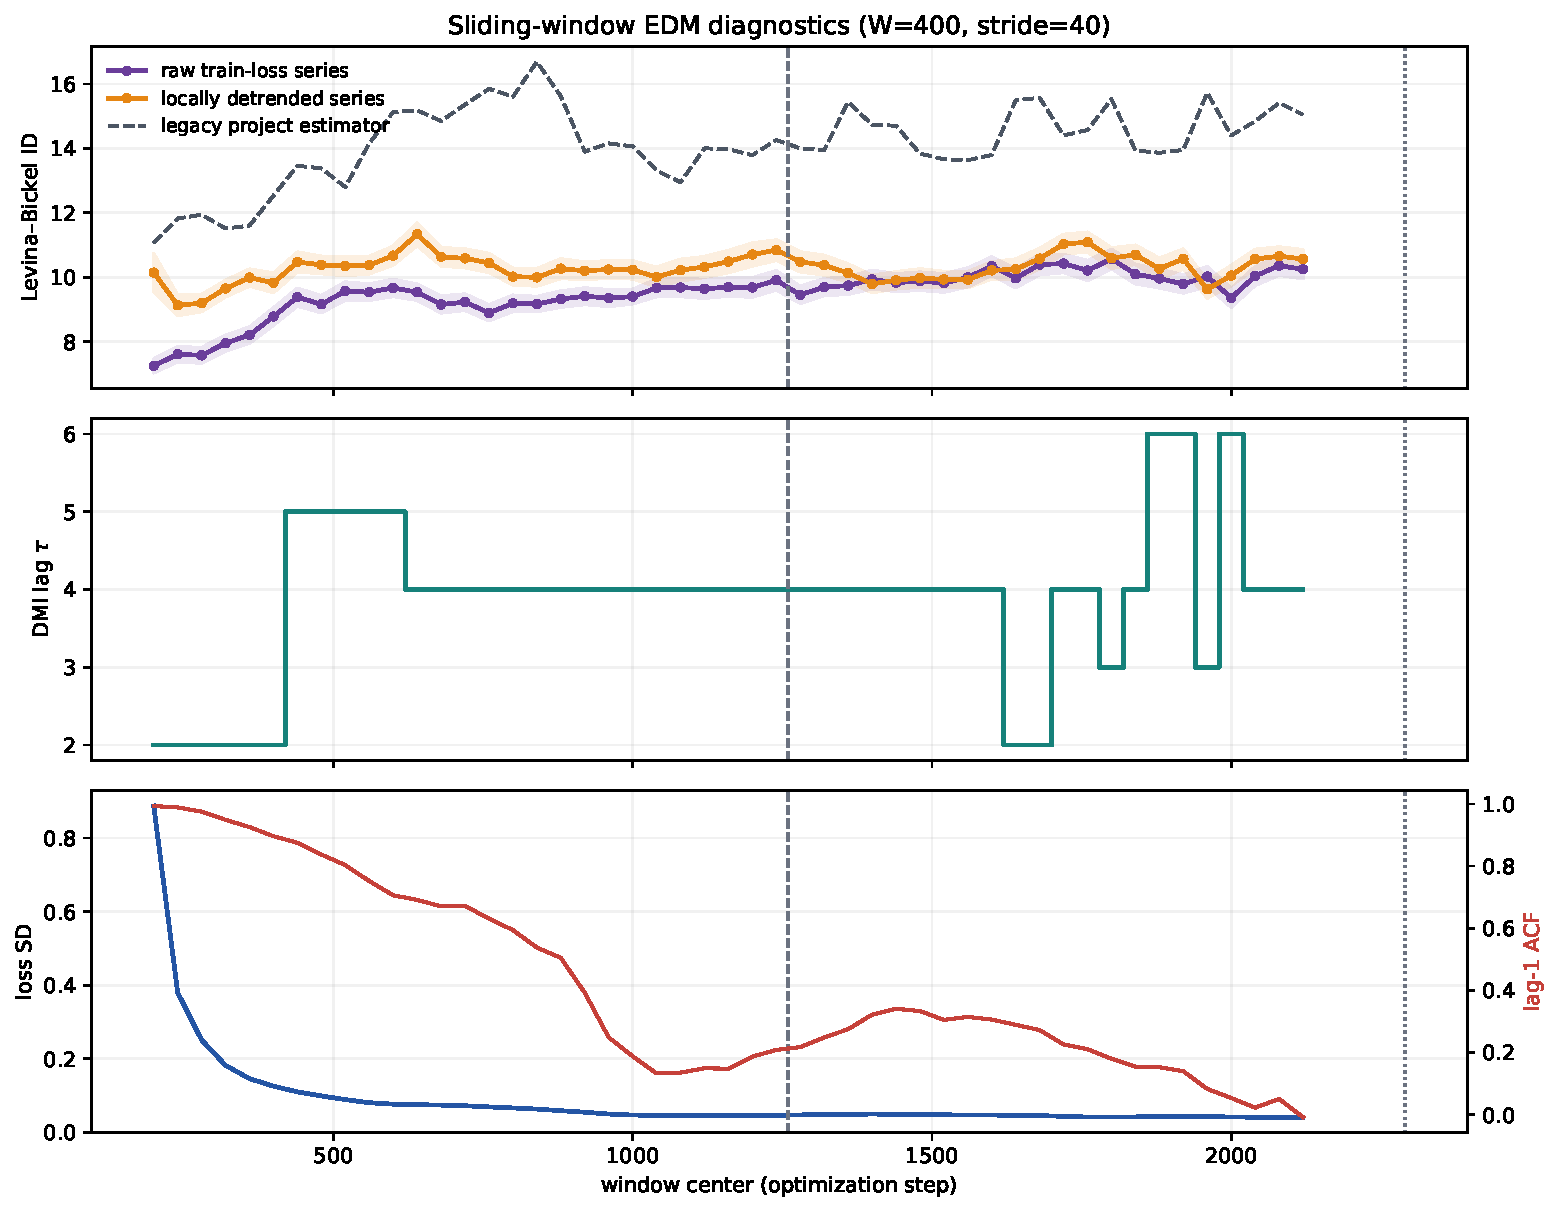
\includegraphics[width=\textwidth]{02_edm_trajectory.pdf}
  \caption{Скользящие оценки размерности, выбранный DMI lag и статистики loss.}
\end{figure}

\section{Результаты}

Для сырого ряда средняя оценка первых 12 окон равна 8.69, последних 12 окон ---
10.12. Для detrended ряда соответствующие значения равны 10.13 и 10.52.
Таким образом, ни один вариант не показывает ожидаемого позднего коллапса.

Самая низкая сырая оценка, 7.25, наблюдается в окне с центром на шаге 200. Но
lag-1 autocorrelation в этом окне равна 0.993, а после detrending ID возрастает
до 10.14. Следовательно, ранняя низкая размерность обусловлена глобальным
трендом, а не компактным поздним состоянием оптимизатора.

\begin{table}[ht]
\centering
\caption{Средние скользящие оценки по фазам schedule.}
\begin{tabular}{lrrrrr}
\toprule
Фаза & Центры окон & $\tau$ & ID raw & ID detrended & Legacy ID \\
\midrule
Constant LR & 200--1240 & 4 & $9.10\pm0.73$ & $10.25\pm0.46$ & $13.81\pm1.46$ \\
LR cooldown & 1280--2120 & 4 & $10.01\pm0.31$ & $10.33\pm0.39$ & $14.57\pm0.72$ \\
\bottomrule
\end{tabular}
\end{table}

\begin{figure}[ht]
  \centering
  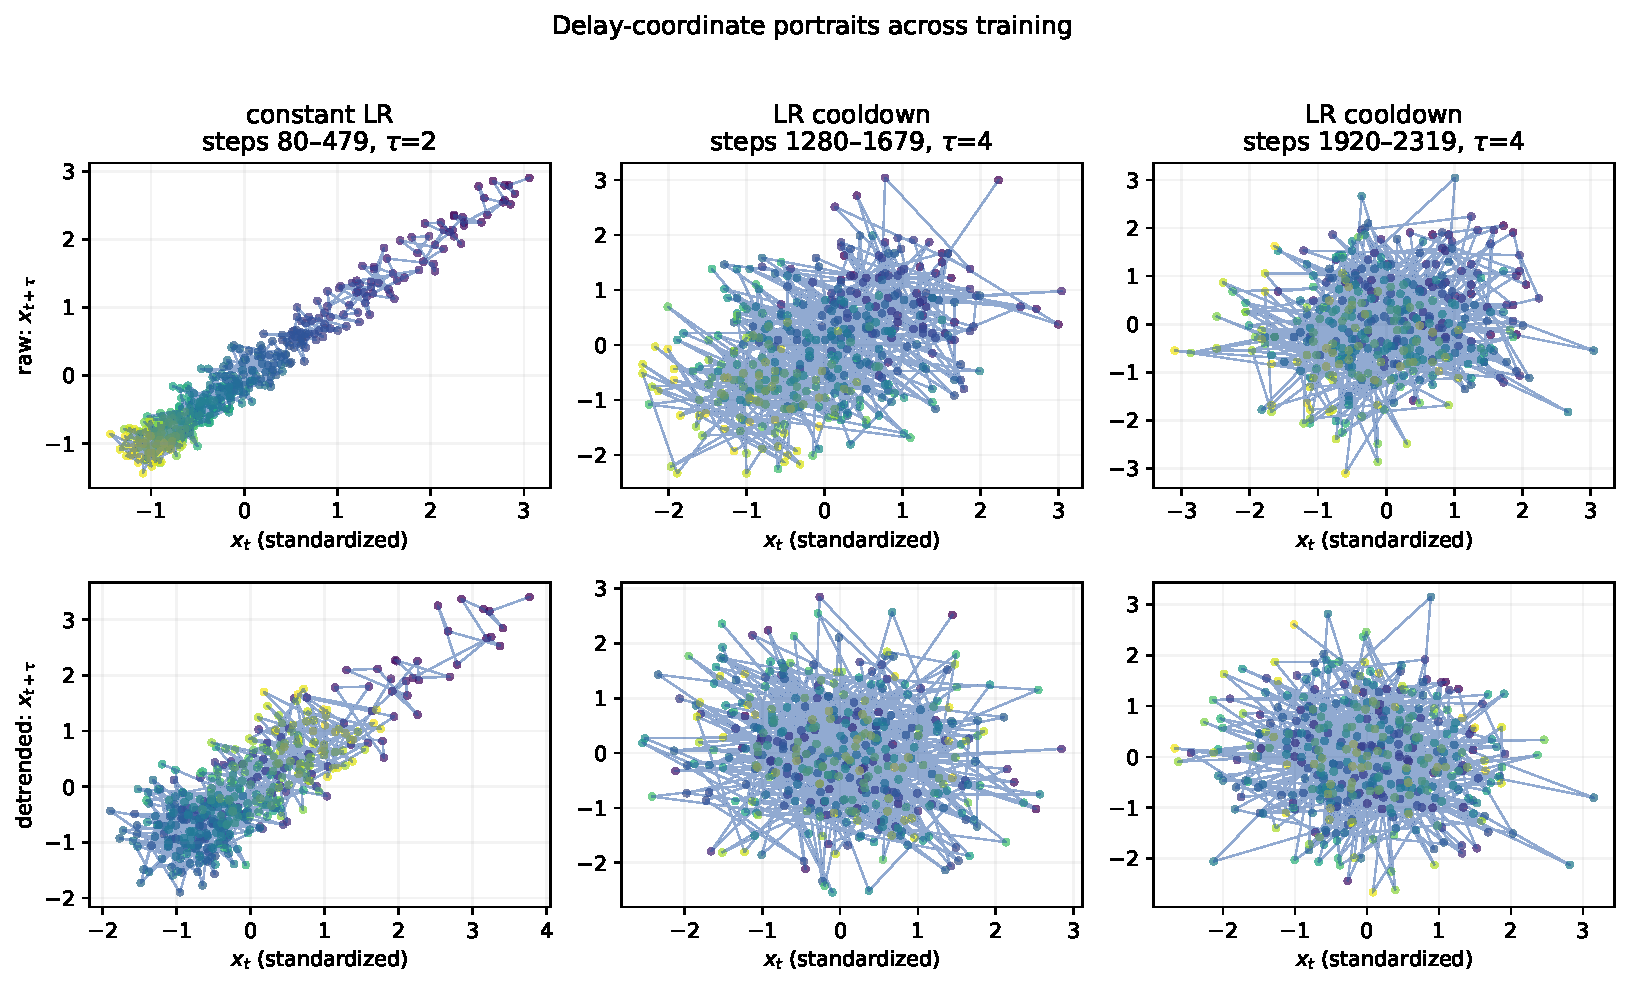
\includegraphics[width=\textwidth]{03_phase_portraits.pdf}
  \caption{Delay-coordinate portraits в ранней, средней и поздней частях обучения.}
\end{figure}

\section{Проверка устойчивости}

Расчёт повторён для окон 300, 400, 500 и 600 и задержек 1, 2, 3, 5 и 8.
Поздняя оценка не становится устойчиво ниже ранней. Для detrended loss диапазоны
составляют 7.7--10.3 (early), 10.0--11.1 (middle) и 9.5--11.3 (late).

\begin{figure}[ht]
  \centering
  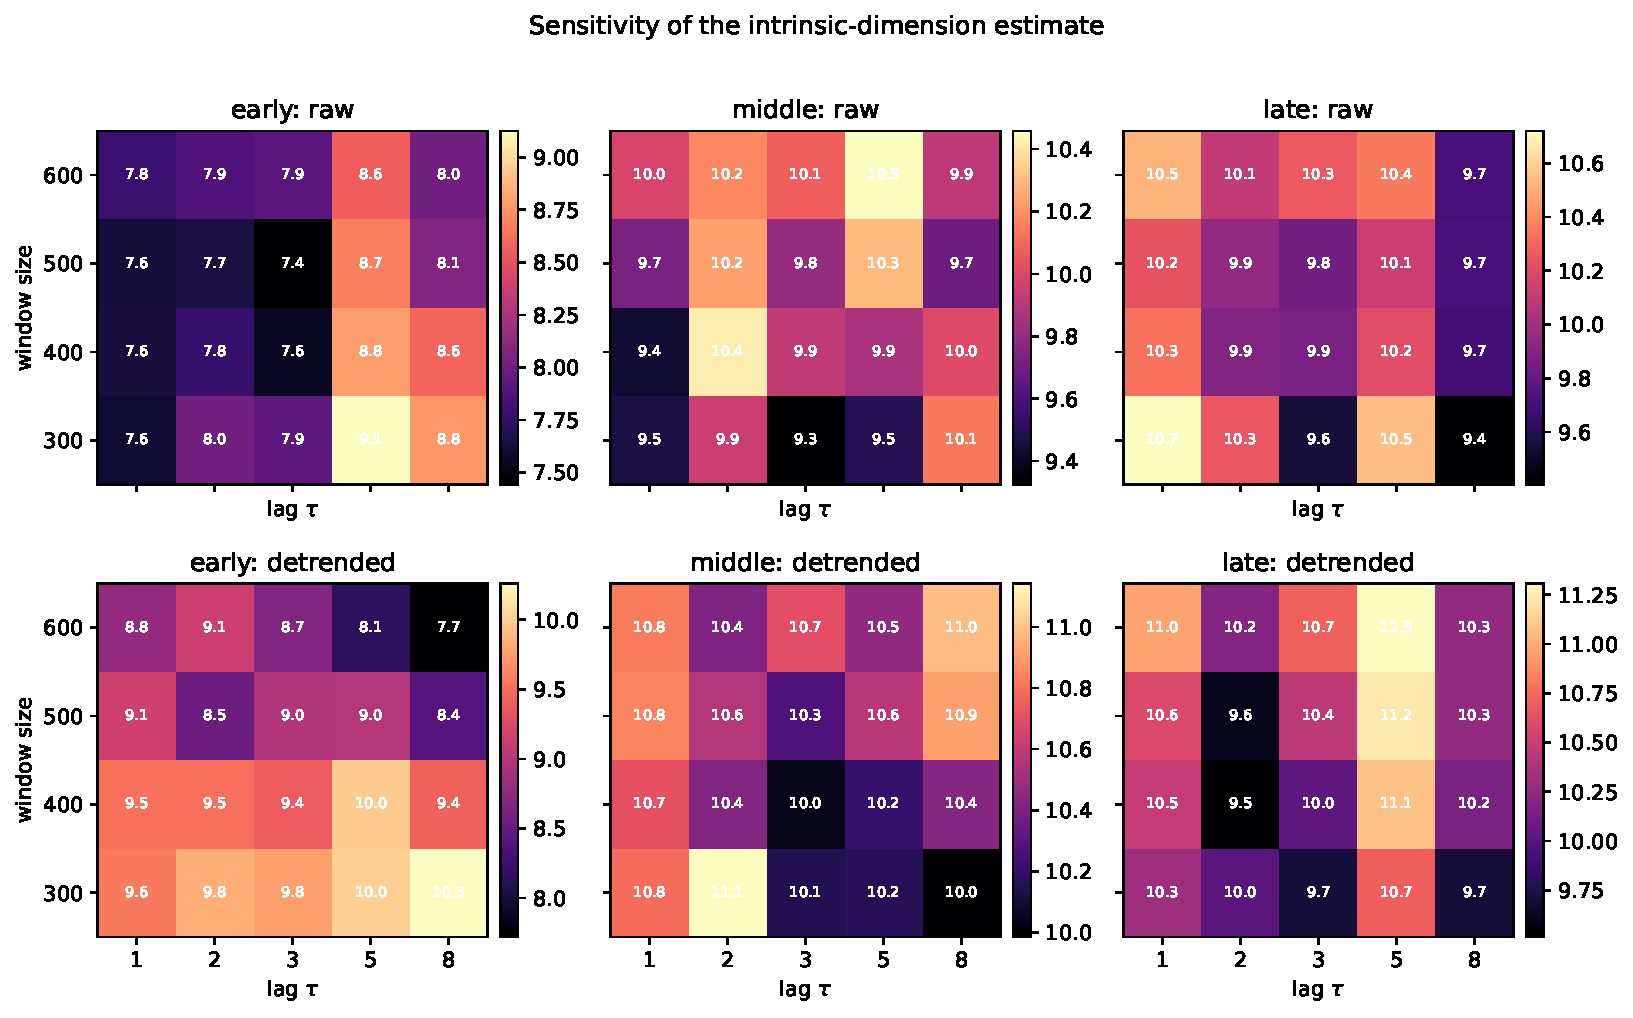
\includegraphics[width=\textwidth]{04_robustness.pdf}
  \caption{Чувствительность оценки к размеру окна и задержке.}
\end{figure}

Оценка зависит и от размерности пространства реконструкции, приближаясь при
$m=12$ к верхней границе. Поэтому значения 10--10.5 нельзя считать точной
физической размерностью; надёжным является сравнительный вывод об отсутствии
выраженного позднего коллапса.

\begin{figure}[ht]
  \centering
  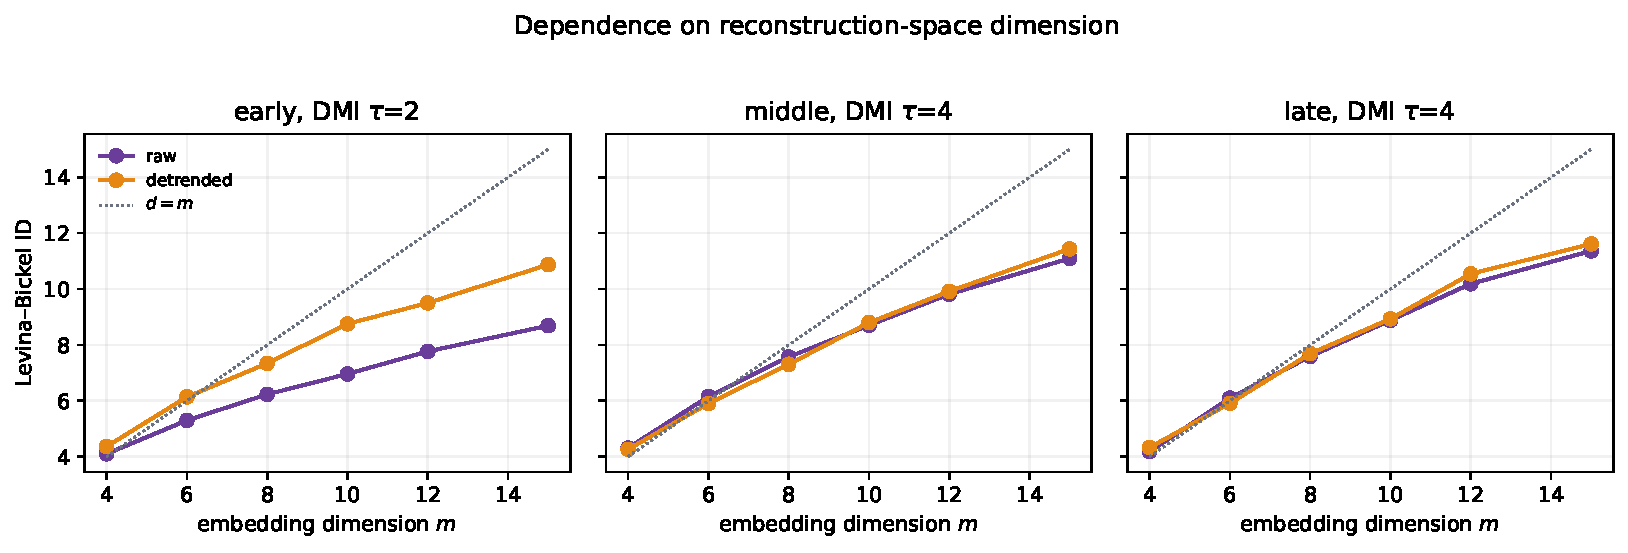
\includegraphics[width=\textwidth]{05_embedding_sensitivity.pdf}
  \caption{Зависимость MLE ID от размерности delay embedding.}
\end{figure}

\section{Интерпретация и ограничения}

Эксперимент не содержит plateau между memorization и delayed generalization:
train и validation loss непрерывно снижаются, а accuracy не логируется. Кроме
того, learning-rate schedule делает процесс нестационарным. Доступен один запуск,
один плотный observable и нет контрольных seed или других оптимизаторов.

Поэтому полученный результат полезен как negative/control case: успешное
обучение большой языковой модели само по себе не обязано сопровождаться
dimensionality collapse в скалярном loss. Для сравнительного исследования нужны
логи остальных методов (MuonUSign, EF21-*, SignMuon, MuonSign, SignSGD) и
несколько seed. Разработанный парсер и анализатор готовы к их обработке.

\end{document}
